\begin{figure}[t]
  \centering
  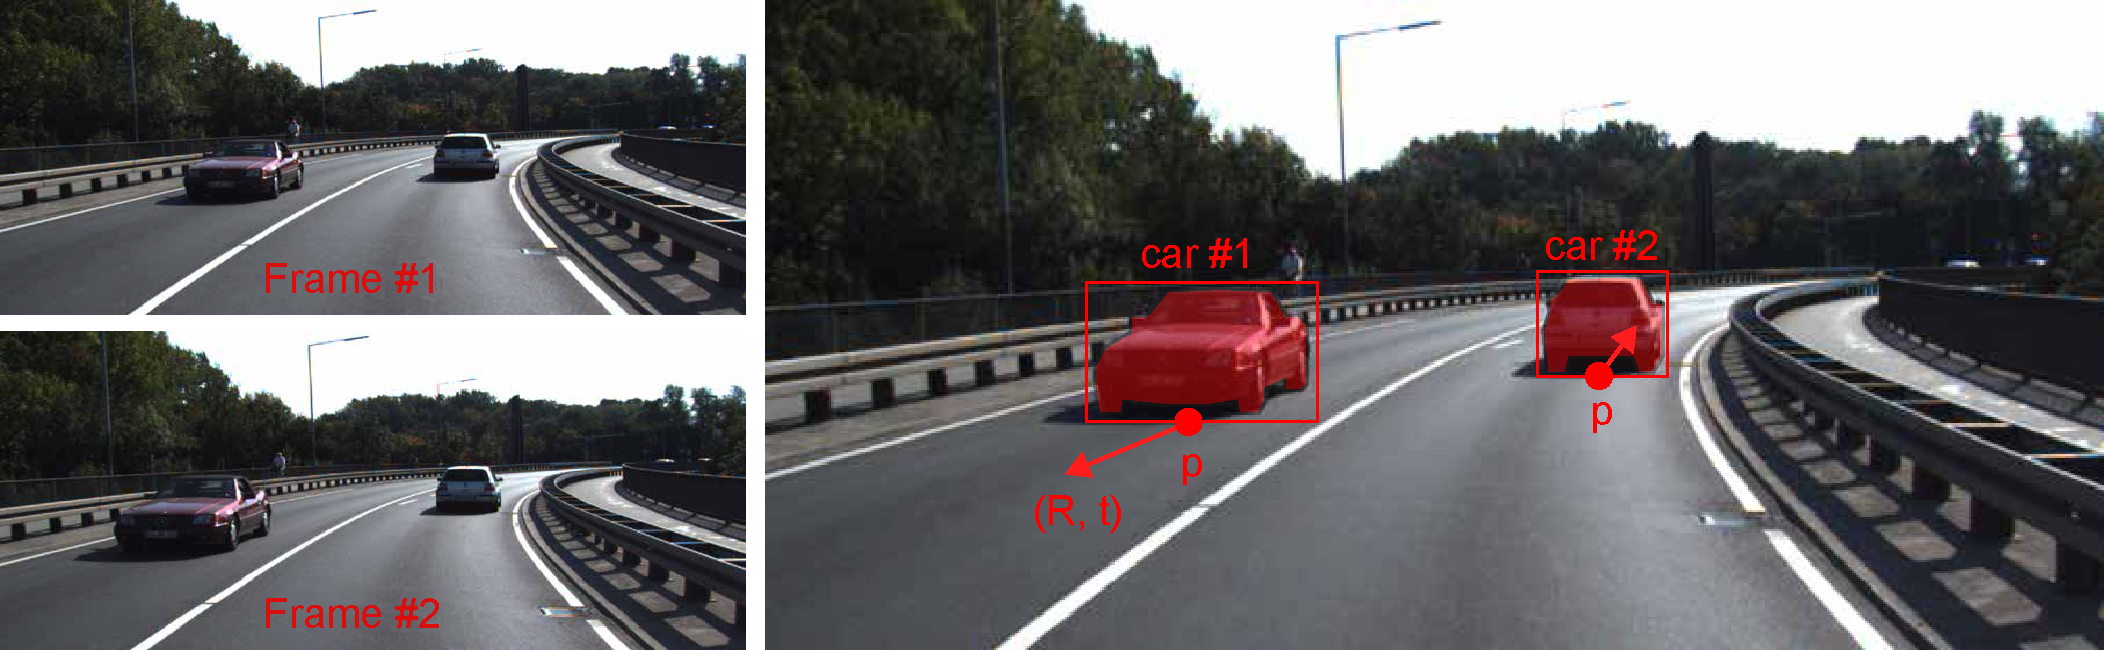
\includegraphics[width=\textwidth]{figures/teaser}
\caption{
Given two temporally consecutive frames,
our network segments the pixels of the first frame into individual objects
and estimates their 3D locations as well as all 3D object motions between the frames.
}
\label{figure:teaser}
\end{figure}

\subsection{Motivation}

For moving in the real world, it is generally desirable to know which objects exists
in the proximity of the moving agent,
where they are located relative to the agent,
and where they will be at some point in the future.
In many cases, it would be preferable to infer such information from video data
if technically feasible, as camera sensors are cheap and ubiquitous.

For example, in autonomous driving, it is crucial to not only know the position
of each obstacle, but to also know if and where the obstacle is moving,
and to use sensors that will not make the system too expensive for widespread use.

A promising approach for 3D scene understanding in situations like these are deep neural
networks, which have recently achieved breakthroughs in object detection, instance segmentation and classification
in still images and are more and more often being applied to video data.
A key benefit of end-to-end deep networks is that they can, in principle,
enable very fast inference on real time video data and generalize
over many training examples to resolve ambiguities inherent in image understanding
and motion estimation.

Thus, in this work, we aim to develop end-to-end deep networks which can, given
sequences of images, segment the image pixels into object instances and estimate
the location and 3D motion of each object instance relative to the camera
(Figure \ref{figure:teaser}).

\subsection{Technical goals}

Recently, SfM-Net \cite{SfmNet} introduced an end-to-end deep learning approach for predicting depth
and dense optical flow in monocular image sequences based on estimating the 3D motion of individual objects and the camera.
SfM-Net predicts a batch of binary full image masks specyfing the object memberships of individual pixels with a standard encoder-decoder
network for pixel-wise prediction. A fully-connected network branching off the encoder predicts a 3D motion for each object.
However, due to the fixed number of objects masks, the system can only predict a small number of motions and
often fails to properly segment the pixels into the correct masks or assigns background pixels to object motions (Figure \ref{figure:sfmnet_kitti}).
\begin{figure}[t]
  \centering
  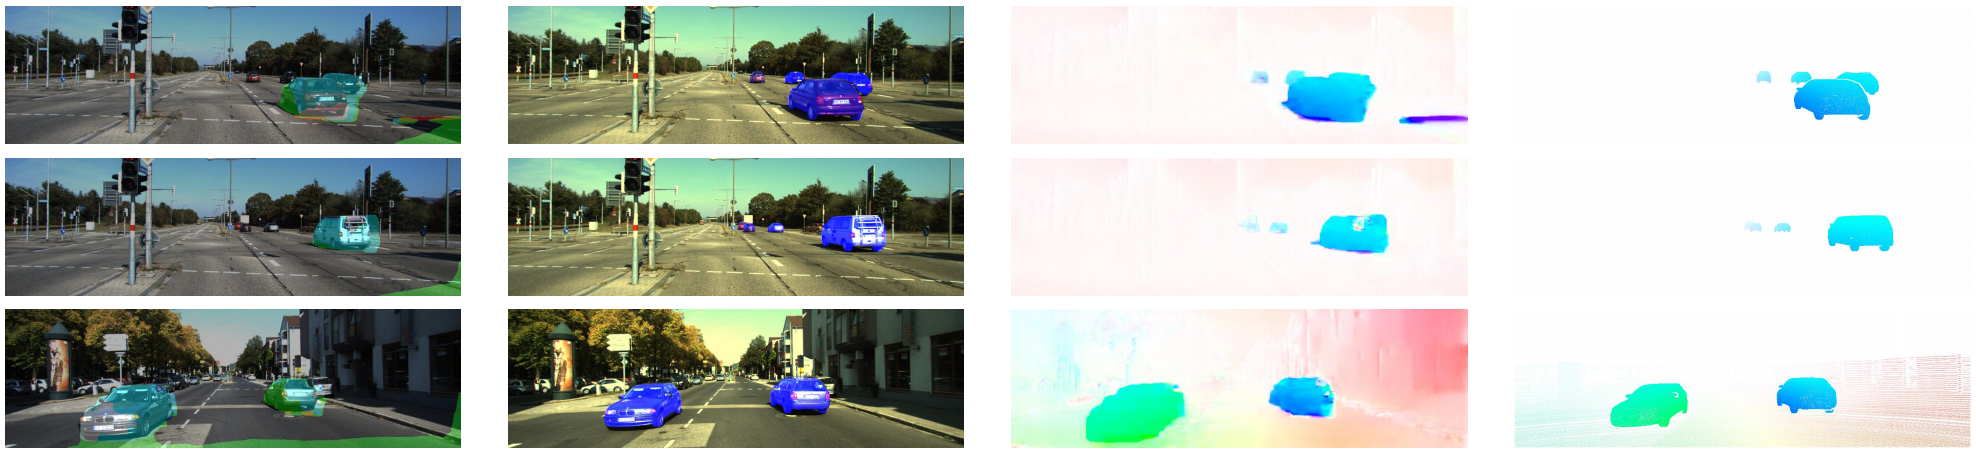
\includegraphics[width=\textwidth]{figures/sfmnet_kitti}
\caption{
Results of SfM-Net \cite{SfmNet} on KITTI \cite{KITTI2015}.
From left to right we show, instance segmentation into up to 3 independent objects,
ground truth instance masks for the segmented objects, composed optical flow and ground truth optical flow.
Figure from \cite{SfmNet}.
}
\label{figure:sfmnet_kitti}
\end{figure}
Thus, this approach is very unlikely to scale to dynamic scenes with a potentially
large number of diverse objects due to the inflexible nature of their instance segmentation technique.

A scalable approach to instance segmentation based on region-based convolutional networks
was recently introduced with Mask R-CNN \cite{MaskRCNN}, which inherits the ability to detect
a large number of objects from a large number of classes at once from Faster R-CNN
and predicts pixel-precise segmentation masks for each detected object (Figure \ref{figure:maskrcnn_cs}).

\begin{figure}[t]
  \centering
  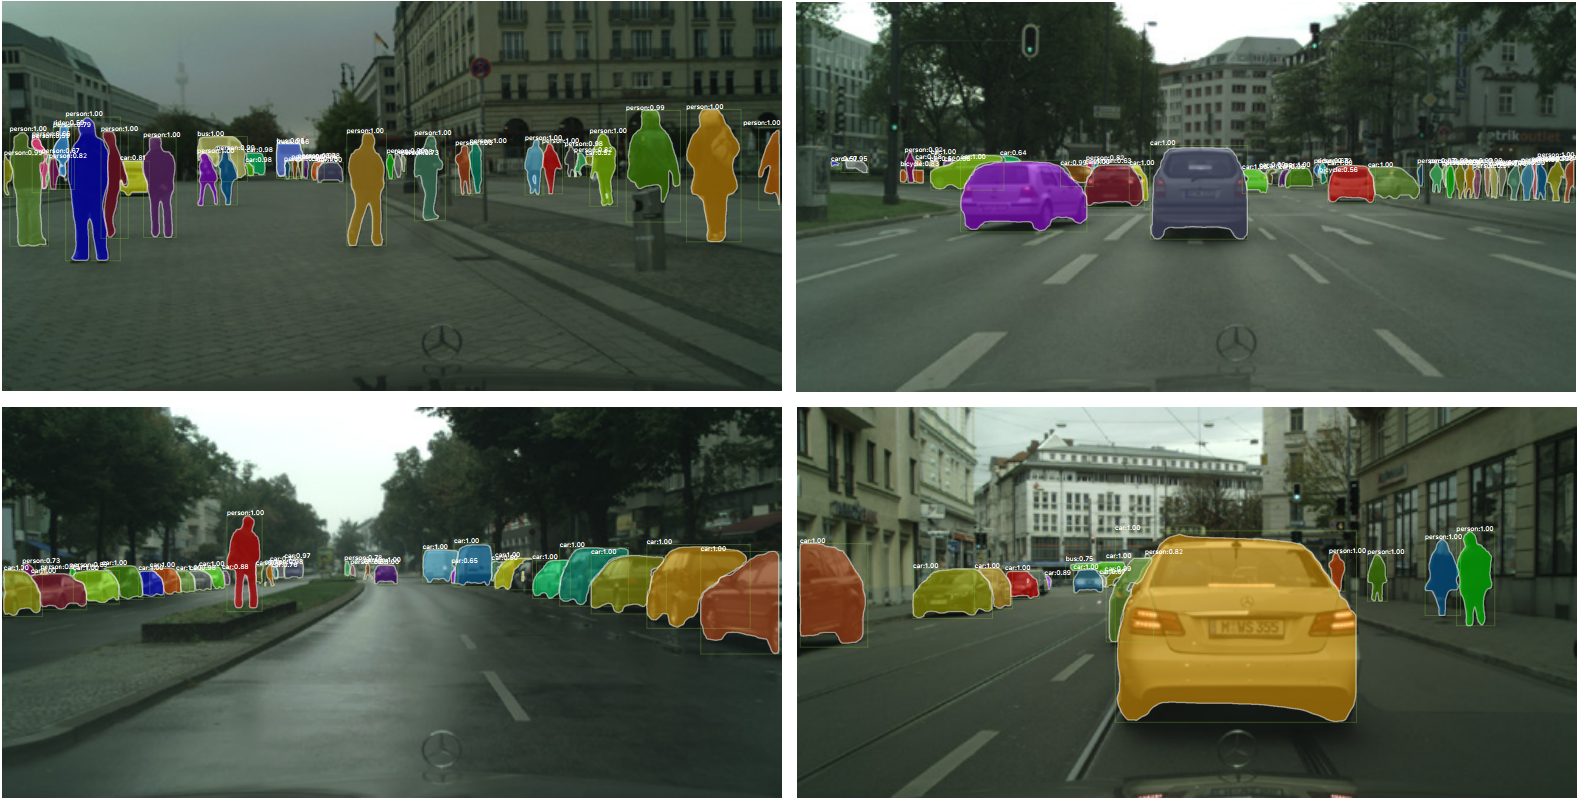
\includegraphics[width=\textwidth]{figures/maskrcnn_cs}
\caption{
Instance segmentation results of Mask R-CNN ResNet-50-FPN \cite{MaskRCNN}
on Cityscapes \cite{Cityscapes}. Figure from \cite{MaskRCNN}
}
\label{figure:maskrcnn_cs}
\end{figure}

We propose \emph{Motion R-CNN}, which combines the scalable instance segmentation capabilities of
Mask R-CNN with the end-to-end 3D motion estimation approach introduced with SfM-Net.
For this, we naturally integrate 3D motion prediction for individual objects into the per-RoI R-CNN head
in parallel to classification, bounding box refinement and mask prediction.
For each RoI, we predict a single 3D rigid object motion together with the object
pivot in camera space in this way.
As a foundation for image matching, we extend the ResNet \cite{ResNet} backbone of Mask R-CNN to take
two concatenated images as input, similar to FlowNetS \cite{FlowNet}.
This results in a fully integrated end-to-end network architecture for segmenting pixels into instances
and estimating the motion of all detected instances without any limitations
as to the number or variety of object instances (Figure \ref{figure:net_intro}).

Eventually, we want to extend our method to include depth prediction,
yielding the first end-to-end deep network to perform 3D scene flow estimation
in a principled way from considering individual objects.
For now, we will work with RGB-D frames to break down the problem into
manageable pieces.

\begin{figure}[t]
  \centering
  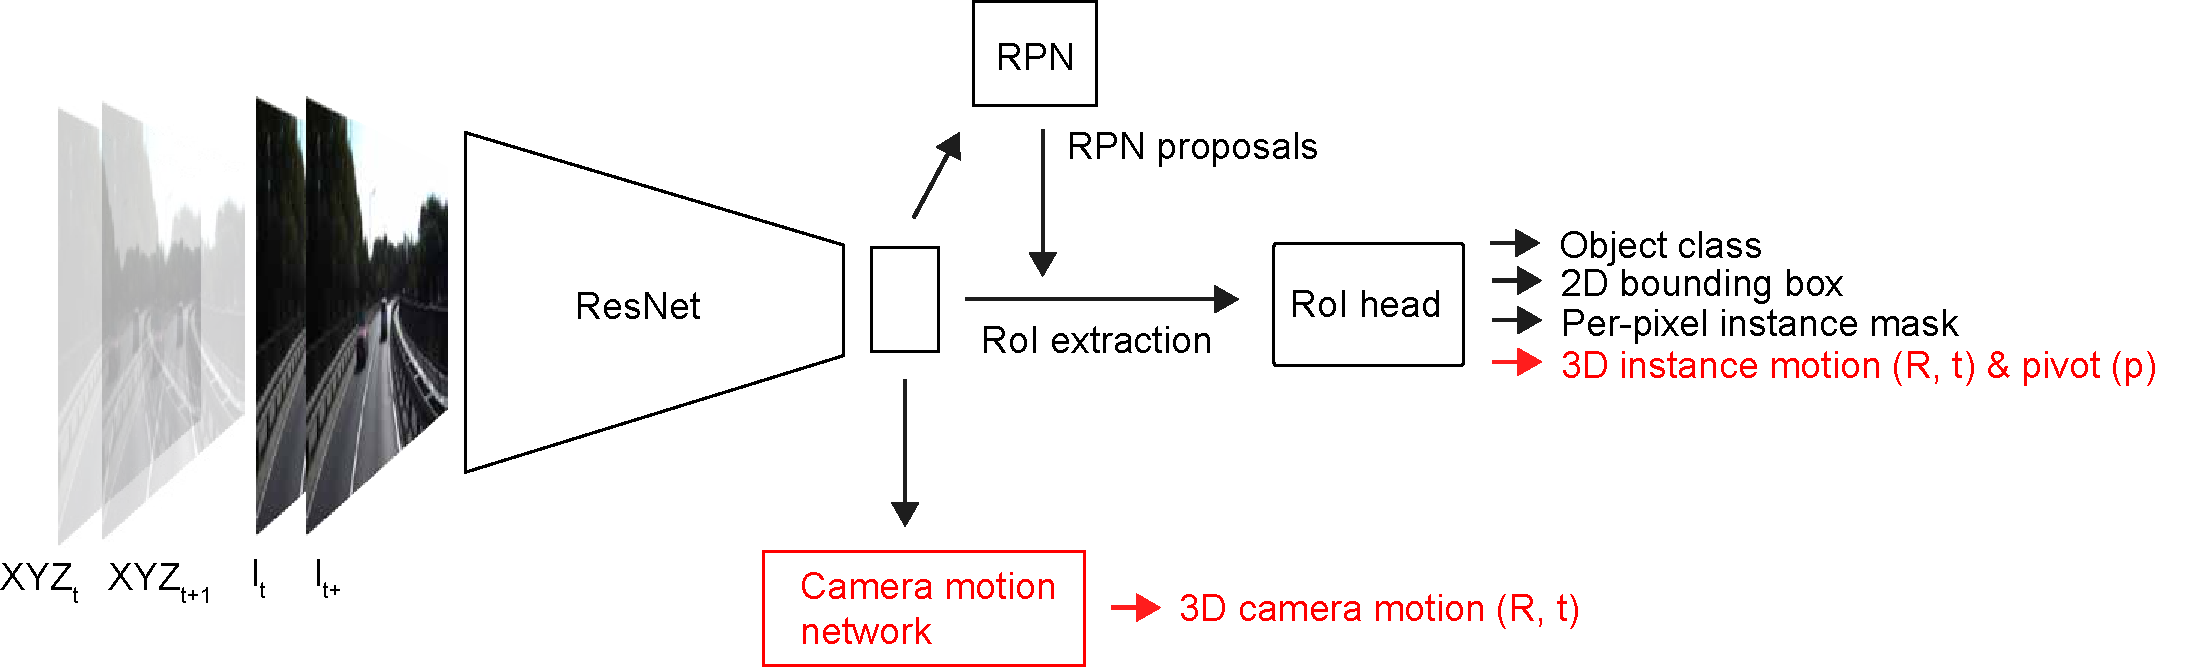
\includegraphics[width=\textwidth]{figures/net_intro}
\caption{
Overview of our network based on Mask R-CNN. For each RoI, we predict the instance motion
in parallel to the class, bounding box and mask. We branch off a additionaly
small network for predicting the camera motion from the bottleneck.
}
\label{figure:net_intro}
\end{figure}

\subsection{Related work}

In the following, we will refer to systems which use deep networks for all
optimization and do not perform time-critical side computation at inference time as
\emph{end-to-end} deep learning systems.

\paragraph{Deep networks in optical flow}

End-to-end deep networks for optical flow were recently introduced
based on encoder-decoder networks or CNN pyramids \cite{FlowNet, FlowNet2, SPyNet},
which pose optical flow as generic, homogenous pixel-wise estimation problem without making any assumptions
about the regularity and structure of the estimated flow.
Specifically, such methods ignore that the optical flow varies across an
image depending on the semantics of each region or pixel, which include whether a
pixel belongs to the background, to which object instance it belongs if it is not background,
and the class of the object it belongs to.
Often, failure cases of these methods include motion boundaries or regions with little texture,
where semantics become more important. \todo{elaborate}% TODO make sure this is a grounded statement
Extensions of these approaches to scene flow estimate flow and depth
with similarly generic networks \cite{SceneFlowDataset} and similar limitations.

Other works \cite{FlowLayers, ESI, MRFlow} make use of semantic segmentation to structure % TODO cite jun's paper?
the optical flow estimation problem and introduce reasoning at the object level,
but still require expensive energy minimization for each
new input, as CNNs are only used for some of the components.

In contrast, we tackle motion estimation at the instance-level with end-to-end
deep networks and derive optical flow from the individual object motions.

\paragraph{Slanted plane methods for 3D scene flow}
The slanted plane model for scene flow \cite{PRSF, PRSM} models a 3D scene as being
composed of planar segments. Pixels are assigned to one of the planar segments,
each of which undergoes a independent 3D rigid motion. % TODO explain benefits of this modelling, but unify with explanations above
In contrast to \cite{PRSF, PRSM}, the Object Scene Flow method \cite{KITTI2015}
assigns each slanted plane to one rigidly moving object instance, thus
reducing the number of independently moving segments by allowing multiple
segments to share the motion of the object they belong to.
In all of these methods, pixel assignment and motion estimation are formulated
as energy-minimization problem which is optimized for each input data point,
without the use of (deep) learning. % TODO make sure it's ok to say there's no learning

In a more recent approach termed Instance Scene Flow \cite{InstanceSceneFlow},
a CNN is used to compute 2D bounding boxes and instance masks for all objects in the scene, which are then combined
with depth obtained from a non-learned stereo algorithm to be used as pre-computed
inputs to a slanted plane scene flow model based on \cite{KITTI2015}.
Most likely due to their use of deep learning for instance segmentation and for some other components, this
approach outperforms the previous related scene flow methods on public benchmarks.
Still, the method uses a energy-minimization formulation for the scene flow estimation
and takes minutes to make a prediction.

Interestingly, the slanted plane methods achieve the current state-of-the-art
in scene flow \emph{and} optical flow estimation on the challenging KITTI benchmarks \cite{KITTI2012, KITTI2015},
outperforming end-to-end deep networks like \cite{FlowNet2, SceneFlowDataset}.
However, the end-to-end deep networks are significantly faster than their energy-minimization counterparts,
generally taking a fraction of a second instead of minutes for prediction and can often be made to run in realtime.
These concerns restrict the applicability of the current slanted plane models in practical settings,
which often require estimations to be done in realtime and for which an end-to-end
approach based on learning would be preferable.

Futhermore, in other contexts, the move towards end-to-end deep learning has often lead
to significant benefits in terms of accuracy and speed.
As an example, consider the evolution of region-based convolutional networks, which started
out as prohibitively slow with a CNN as a single component and
became very fast and much more accurate over the course of their development into
end-to-end deep networks.

Thus, in the context of motion estimation, one could expect end-to-end deep learning to not only bring large improvements
in speed, but also in accuracy, especially considering the inherent ambiguity of motion estimation
and the ability of deep networks to learn to handle ambiguity from a large variety of training examples.

However, we think that the current end-to-end deep learning approaches to motion
estimation are likely limited by a lack of spatial structure and regularity in their estimates
as explained above, which stems from the generic nature of the employed networks.
To this end, we aim to combine the modelling benefits of rigid scene decompositions
with the promise of end-to-end deep learning.

\paragraph{End-to-end deep networks for 3D rigid motion estimation}
End-to-end deep learning for predicting rigid 3D object motions was first introduced with
SE3-Nets \cite{SE3Nets}, which take raw 3D point clouds as input and produce a segmentation
of the points into objects together with the 3D motion of each object.
Bringing this idea to the context of image sequences, SfM-Net \cite{SfmNet} takes two consecutive frames and
estimates a segmentation of pixels into objects together with their 3D motions between the frames.
In addition, SfM-Net predicts dense depth and camera motion to obtain full 3D scene flow from end-to-end deep learning.
For supervision, SfM-Net penalizes the dense optical flow composed from all 3D motions and the depth estimate
with a brightness constancy proxy loss.

Like SfM-Net, we aim to estimate motion and instance segmentation jointly with
end-to-end deep learning.
Unlike SfM-Net, we build on a scalable object detection and instance segmentation
approach with R-CNNs, which provide a strong baseline.

\paragraph{End-to-end deep networks for camera pose estimation}
Deep networks have been used for estimating the 6-DOF camera pose from
a single RGB frame \cite{PoseNet, PoseNet2}. These works are related to
ours in that we also need to output various rotations and translations from a deep network
and thus need to solve similar regression problems and use similar parametrizations
and losses.


\subsection{Outline}
In section \ref{sec:background}, we introduce preliminaries and building
blocks from earlier works that serve as a foundation for our networks and losses.
Most importantly, we re-view the ResNet CNN (\ref{ssec:resnet}) that will serve as CNN backbone
as well as the developments in region-based CNNs onto which we build (\ref{ssec:rcnn}),
specifically Mask R-CNN and the FPN \cite{FPN}.
In section \ref{sec:approach}, we describe our technical contribution, starting
with our modifications to the Mask R-CNN backbone and head networks (\ref{ssec:architecture}),
followed by our losses and supervision methods for training
the extended region-based CNN (\ref{ssec:supervision}), and
finally the postprocessings we use to derive dense flow from our 3D motion estimates
(\ref{ssec:postprocessing}).
In section \ref{sec:experiments}, we introduce the Virtual KITTI dataset we use
for training our networks as well as all preprocessings we perform (\ref{ssec:datasets}),
give details of our experimental setup (\ref{ssec:setup}),
and finally describe the experimental results
on Virtual KITTI (\ref{ssec:vkitti}).
In section \ref{sec:conclusion}, we summarize our work and describe future
developments, including depth prediction, training on real world data,
and exploiting frames over longer time intervals.
